\documentclass[11pt,twocolumn]{article}

%%%%%%%%%%%%%%%%%%%%___ PACKAGES ___%%%%%%%%%%%%%%%
%%%%%%%%%%%%%%%%%%%%%%%%%%%%%%%%%%%%%%%%%%%%%%%%%%%

	\usepackage{amsmath, amssymb}
	\usepackage{microtype}
	\usepackage{empheq}
	\usepackage{siunitx}
	\usepackage{dsfont}

	% \usepackage{ebgaramond-maths}
	% \usepackage[T1]{fontenc}

	\usepackage[tmargin=0.7in, bmargin=0.8in, lmargin=0.5in, rmargin=0.5in]{geometry}

	\usepackage{tikz}
	\usetikzlibrary{patterns,arrows,decorations.pathreplacing,hobby}
	\usepackage{graphicx}
	\usepackage{caption}
	\usepackage{subcaption}

	\definecolor{lightblue}{RGB}{73,151,208}
	\definecolor{crimson}{RGB}{218,61,73}

%%%%%%%%%%%%%%%%%%%%___ COMMANDS ___%%%%%%%%%%%%%%%
%%%%%%%%%%%%%%%%%%%%%%%%%%%%%%%%%%%%%%%%%%%%%%%%%%%

	\newcommand{\cit}{\textbf{[$\blacksquare$] }}
	\newcommand*\mystrut[1]{\vrule width0pt height0pt depth#1\relax}

	\makeatletter
	\renewcommand*\env@matrix[1][\arraystretch]{%
		\edef\arraystretch{#1}%
		\hskip -\arraycolsep
		\let\@ifnextchar\new@ifnextchar
		\array{*\c@MaxMatrixCols c}}
	\makeatother

	% \setlength{\belowdisplayskip}{0pt} \setlength{\belowdisplayshortskip}{0pt}
	% \setlength{\abovedisplayskip}{0pt} \setlength{\abovedisplayshortskip}{0pt}
	\setlength{\columnsep}{1cm}
	\setlength{\parskip}{0cm}
	\setlength{\parindent}{0.75cm}

\begin{document}

%%%%%%%%%%%%%%%%%%%%___ TITLE ___%%%%%%%%%%%%%%%%%%
%%%%%%%%%%%%%%%%%%%%%%%%%%%%%%%%%%%%%%%%%%%%%%%%%%%

	\title{Characterizing Computational Techniques for Experimentally Feasible Non-Local Evolution of Two-Qubit Systems}
	\author{Shankar \textsc{Balasubramanian}\;\; Didi \textsc{Chang-Park}\;\; Kyle \textsc{Herndon}\;\; Zane \textsc{Rossi}}
	\date{}


%%%%%%%%%%%%%%%%%%%%___ ABSTRACT ___%%%%%%%%%%%%%%%
%%%%%%%%%%%%%%%%%%%%%%%%%%%%%%%%%%%%%%%%%%%%%%%%%%%

	\twocolumn[
	  \begin{@twocolumnfalse}
	    \maketitle
	    \begin{abstract}
	    This paper investigates computational methods and presents a computational framework for simulating non-local evolution of two-qubit systems. This evolution may then easily be combined with finite local operations to give control of near-arbitrary precision. Current research has focused on developing the theoretical background which we hope to computationally implement. We will characterize how useful operators (particularly the $CNOT$ gate) are generated in this process, and they will be approximated and performed computationally in optimal time utilizing a adaptive-algorithm approach. We will also analyze the non-local piece of the system Hamiltonian, including determining experimental means of generating it.  Particularly, we will be evaluating its action on the Poincar\'{e}-Bloch-Sphere.
	    \end{abstract}
	    \vspace{2em}
	  \end{@twocolumnfalse}
	]


%%%%%%%%%%%%%%%%%%%%___ INTRO ___%%%%%%%%%%%%%%%%%%
%%%%%%%%%%%%%%%%%%%%%%%%%%%%%%%%%%%%%%%%%%%%%%%%%%%

\section{Introduction}

The ultimate goal of Control Theory is the ability to arbitrarily manipulate the state of an ensemble of qubits \cite{hammerer}. In the context of quantum computation, this problem is reduced further: basic quantum gates allow for modular systems \cite{bremner}. However, the generation of these gates is non-trivial, and the arbitrary Hamiltonian is, in general, not readily constructible. Often one will wish to achieve a specific unitary evolution operator or gate $U$ corresponding to the solitary time evolution of a Hamiltonian $H$. When $H$ may not be engineered easily, the evolution can be achieved in other ways \cite{bremner} , often involving the use of local operations (LO), repeated measurements on the system \cite{bennett}, along with standard Hamiltonian-driven evolution drawing from some collection (possibly a one element collection) $H_1, H_2, \cdots, H_n$, all of which \emph{can} be lucratively generated.

	In the simplest case, a two particle system, the Hamiltonians involved may contain non-local terms, usually corresponding to particle-particle interactions. This paper will propose a framework for taking the general non-local Hamiltonian \cite{bennett} 
	\begin{equation}
	H = A \otimes \mathds{1} + \mathds{1} \otimes B + \sum_{ij} M_{ij}\,  \sigma_i \otimes \sigma_j
	\end{equation}
	and interspersing its non-local part's evolution with LO to achieve a desired $U$. It is only the non-local part of the Hamiltonian which must be studied, and through decomposition of this piece into its canonical form, and some insight into Lie Theory, we are able to formulate a computational approach \cite{haselgrove}. Devising a scheme to generate a $U$ from a collection of available operators and Hamiltonians has direct applicablity to a variety of problems, but cannot be done purely analytically on a massive scale, thus making a computational method necessary.



%%%%%%%%%%%%%%%%%%%%___ SYSCLAS ___%%%%%%%%%%%%%%%%
%%%%%%%%%%%%%%%%%%%%%%%%%%%%%%%%%%%%%%%%%%%%%%%%%%%

	\section{Classifying Systems}

	The schemes introduced for generating a particular operator rely on manipulations in defined spaces that we notate LU, LU$+$, LO, and LO$+$ \cite{bennett}. We are only concerned in manipulation within LU, which refers to unitary operators acting on the space $\left(A\otimes B\right)$, a two particle system.\footnote{LU$+$ refers to the abstraction giving multi-particle systems (in these systems, we act on $\left(A\otimes B'\right)$, where $B'$ is itself some ancillary, multi-particle system.)} This is not the most general system in the context of control theory, but it provides a relatively general basis on which to build intuition and computational protocol.

	It can be demonstrated that, in order to simulate a unitary evolution operator which demonstrates \emph{correlation} between its interior pieces, a combination of a purely non-local Hamiltonian, and purely local operators is sufficient \cite{bennett}. This allows a natural separation in any attempted simulation. The disadvantage of this approach lies in the determination of such local operators to create the new unitary operator when interspersed with a particular evolution operator.  

	% \subsection{Canonical Form}

	%%%%%%%%%%%%%%%%%%%%%%%%%%%%%%%%%%%%%%%%%%%%%%%%%%%%%%%

\subsection{Group Theory Exploitation}

	The entirety of this simulation scheme is done with the pauli basis, and this allows their wonderful properties to be exploited. Given further research, the algorithm would implement group theory concepts in its heuristic, but currently, this idea is only used in data compression, and the breeding/mutation of matrices. 

	The local operations described in the preceding section can be realized as unitary matrices, and, through a process described in \textbf{\ref{arg}.}, described by three angles. Because of this, we can imagine all possible unitary operators as lying on the surface of the 3-Sphere\cite{aerts}. This can be represented pictorially,

	\begin{figure}[htpb]
		\centering
		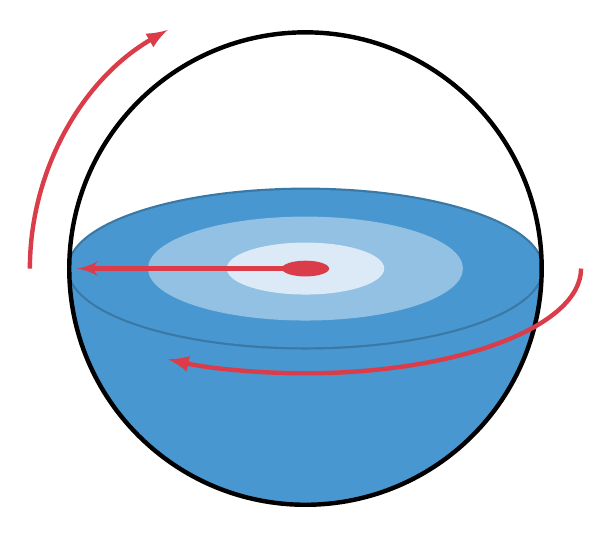
\begin{tikzpicture}[use Hobby shortcut]
		
		\tikzset{
		    partial ellipse/.style args={#1:#2:#3}{
        		insert path={+ (#1:#3) arc (#1:#2:#3)}
    		}
		}

		% clipping for ellipse

		\begin{scope}
			\clip (0,0) circle (3cm);
			\clip (-4,0) rectangle (4,-4);

			\fill[lightblue] (0,0) circle (3cm);
		\end{scope}

		% ellipse drawn
		\draw[ultra thick, lightblue!80!black] (0,0) ellipse (3cm and 1cm);

		\fill[lightblue] (0,0) ellipse (3cm and 1cm);

		\fill[lightblue!60!white] (0,0) ellipse (2cm and 0.66cm);

		\fill[lightblue!20!white] (0,0) ellipse (1cm and 0.33cm);

		% markings and text

		\draw[ultra thick] (0,0) circle (3cm);

		\draw[ultra thick, crimson, -latex] (0,0) [partial ellipse=0:-120:3.5cm and 1.33cm];
		\draw[ultra thick, crimson, -latex] (0,0) [partial ellipse=180:120:3.5cm and 3.5cm];
		\fill[crimson] (0,0) ellipse (0.3cm and 0.1cm);
		\draw[ultra thick, crimson, -latex'] (-0.1,0) -- (-2.9, 0);

		%\draw[ultra thick, crimson, ->] (-4, -0.5).. (-4.25, -0.45) .. (-5, 1) .. (-4, 0.5);



		\end{tikzpicture}
		\centering
		\caption{A pictorial representation of the 3-sphere: the upper half has been removed for clarity. The three arrows represent the degrees of freedom along the 3-sphere's surface, the points of which have been projected to the interior of a 2-sphere. (The arrow along the traditional `radius', if extended, gives degeneracy). Despite implication there is no preferred direction along which to move across the 3-sphere.}
	\end{figure}

	and analyzed for use in the context of an adaptive algorithm. The surface of the 3-Sphere has here been projected to the interior of a 2-Sphere. One could thus imagine a perturbation away from a point on the interior (where movement `out' of the sphere implies returning to the center: a degeneracy)--these are the mutations for our adaptive algorithm. One could also imagine taking a point between two points inside this diagram--this is a rough heuristic for the breeding of two unitary operators (in reality, the geometry is more exotic than a straight average).

%%%%%%%%%%%%%%%%%%%%___ COMPUTE ___%%%%%%%%%%%%%%%%
%%%%%%%%%%%%%%%%%%%%%%%%%%%%%%%%%%%%%%%%%%%%%%%%%%%

	\section{Methods for Computation}

	We now will classify the interface of the theory presented above with modern computational techniques. The particular method used aligns with that of adaptive algorithms: in particular, we have a non-deterministic algorithm which converges on an optimal solution given repeated trials. 

	%%%%%%%%%%%%%%%%%%%%%%%%%%%%%%%%%%%%%%%%%%%%%%%%%%%%%%%

	\subsection{Overview}

	Given the relative abundance of results published concerning the time constraints involved in the simulation of one Hamiltonian by another, devising the concrete method by which one actually pieces together these Hamiltonians is becoming a far more pertinent problem. In general, the scheme for constructing a given unitary evolution operator is through use of alternating free-evolution (FE) under a simple Hamiltonian (represented by a hermitian matrix)

	\begin{equation}
	P = e^{-i H t} \;\;\biggr\vert\;\; H = H^{\dagger}
	\end{equation}

	, and local operations

	\begin{equation}
	Q = A_1 \otimes A_2 \;\;\biggr\vert\;\; A_i^{\dagger}A_i = \mathds{1}
	\end{equation}.

	This may be represented pictorially as a linear sequence.

	\begin{figure}[htpb]
		\centering
		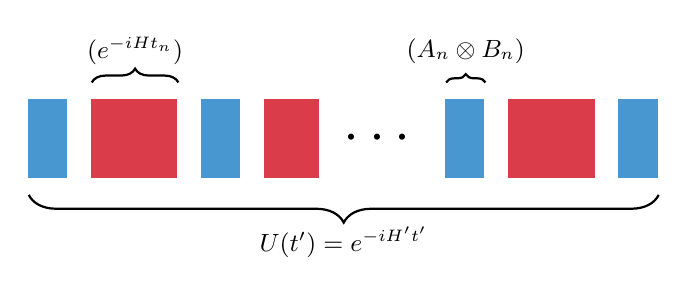
\begin{tikzpicture}

		% evolutions and local operations
		\fill[lightblue] (-4.0, 0) rectangle (-3.5, 1);
		\fill[crimson] (-3.2, 0) rectangle (-2.1, 1);
		\fill[lightblue] (-1.8, 0) rectangle (-1.3, 1);
		\fill[crimson] (-1.0, 0) rectangle (-0.3, 1);

		% dotted continuation
		\node at (0.5 , 0.5) {\huge $\cdots$};

		% more evolutions and local operations
		\fill[lightblue] (4.0, 0) rectangle (3.5, 1);
		\fill[crimson] (3.2, 0) rectangle (2.1, 1);
		\fill[lightblue] (1.8, 0) rectangle (1.3, 1);
		

		% underbrace for overall evolution
		\draw [thick, black, decorate, decoration={brace,amplitude=10pt,mirror}, xshift=0.4pt, yshift=-0.4pt](-4,-0.2) -- (4,-0.2) node[black, midway, yshift=-0.6cm] {\small $U(t') = e^{-iH't'}$};

		% overbrace for hamiltonian
		\draw [thick, black, decorate, decoration={brace,amplitude=5pt}, xshift=0.4pt, yshift=0.4pt](-3.2, 1.2) -- (-2.1, 1.2) node[black, midway, yshift=0.4cm] {\small $(e^{-iHt_n})$};

		% overbrace for local operation
		\draw [thick, black, decorate, decoration={brace,amplitude=3pt}, xshift=0.4pt, yshift=0.4pt](1.3, 1.2) -- (1.8, 1.2) node[black, midway, yshift=0.4cm] {\small $(A_n\otimes B_n)$};

		\end{tikzpicture}
		\centering
		\caption{Representation of generation scheme for a desired unitary evolution operator, $U(t')$.}
	\end{figure}

	We assign the number of steps, $n$, to be a finite integer (for the purposes of tractable computation), and use it to represent the total number of combined free-Hamiltonian/LO bundles. We consider the simulations of $n$-steps to be in an `$n$-family', and will deal with them separately in computation. With this in mind, we can also generalize the case of an infinite number of steps in theory, and have confidence that the simulation will increase in fidelity with this increased `freedom' \cite{hammerer}. 

	%%%%%%%%%%%%%%%%%%%%%%%%%%%%%%%%%%%%%%%%%%%%%%%%%%%%%%%

	\subsection{Adaptive Algorithm Theory}

	Adaptive algorithms thrive on the idea that, in a relatively smooth space, in order to find the optimal solution, following one's nose can work. There are many ways in which this `greed' or `intuition' can be implemented. adaptive algorithms, as evidenced by their names, attempt to mimic the process of evolution by the mechanisms of mutation and natural selection. A set of mathematical objects dubbed \emph{organisms}, each containing some set of data, are subjected to tests against some metric depending on the organism's features \cite{weise}. This is considered one \emph{generation}, and the best organisms of each generation are bred together (by some deterministic algorithm) and mutated to compete in the next generation.

	In preparation for performing a process like the one described, we take three major steps.
	
	To begin, the degrees of freedom of the system should be analyzed, as these will function as the dimensions of the search space. During this process, the degrees which are less pertinent to a solution's fidelity should be identified and their relative mutation amplitude and frequency altered accordingly\footnote{For degrees of freedom analyzed to have less effect on the solution quality, the mutations need not be as quickly decreasing, or as large to begin with. In general, less attention need be given to them.}.

	Next, the mutations assigned to each degree of freedom will be designed so as to best approach a (hopefully) global extrema in the search space. In general, more volatile mutations will be given to the more effective degrees of freedom, and all mutations will decrease in magnitude and frequency as the number of generations increases \cite{satsangi}

	Finally, we need determine the method by which the best organisms of each generation are bred (combined in a way that may retain traits of both.). Note that there is no guarantee under any binary operation that the resulting object will have the same advantages assigned to the parent objects. In the case of well-defined and relatively smooth systems, this breeding will often resemble a sort of average, and the child will often perform similarly to the parents. 

	With these in mind, we can visualize the process as a sort of traversal of a complex multidimensional search space. This will give some heuristic for the arguments for convergence in \textbf{\ref{convergence}.}

	\begin{figure}[htpb]
		\centering
		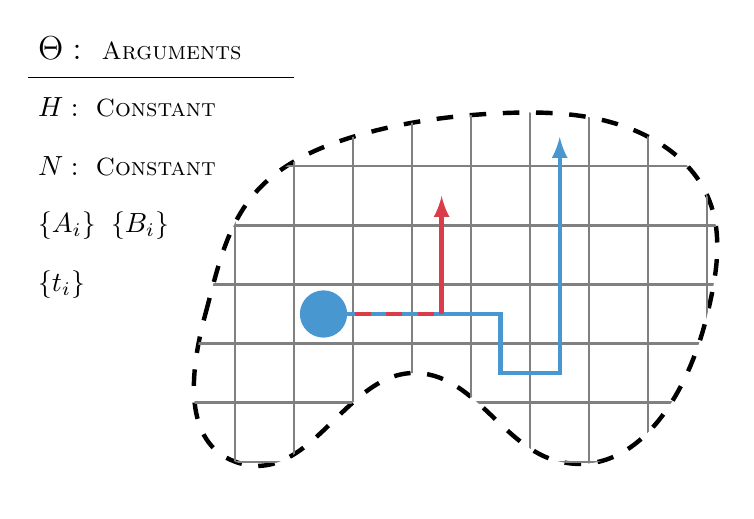
\begin{tikzpicture}[scale=0.75, use Hobby shortcut]

		% main bounding shape
		\draw[ultra thick, closed=true, dash pattern=on 6pt off 6pt] (2.5,4.5) .. (3.3,6.5) .. (5,7.5).. (7.5,7.9).. (10,7.5).. (11,6.5).. (11,4.5) ..(8.5,2).. (6,3.5).. (3,2).. (2.5,4.5);

		%interior grid
		\begin{scope}
			\clip[closed=true] (2.5,4.5) .. (3.3,6.5) .. (5,7.5).. (7.5,7.9).. (10,7.5).. (11,6.5).. (11,4.5) ..(8.5,2).. (6,3.5).. (3,2).. (2.5,4.5);

			\draw[step=1,gray,thick] (0,0) grid (15,15);
		\end{scope}

		% organism paths
		\draw[ultra thick, color=lightblue] (4.5, 4.5) -- (6.5, 4.5);
		\draw[ultra thick, color=crimson, dash pattern=on 0.2cm off 0.2cm] (4.5, 4.5) -- (6.5, 4.5);
		% yeah, that's right, I just did that (dashed overlay)
		\draw[ultra thick, -latex, color=lightblue] (6.5, 4.5) -- (7.5,4.5) -- (7.5,3.5) -- (8.5,3.5) -- (8.5,7.5);
		\draw[ultra thick, -latex, color=crimson] (6.5, 4.5) -- (6.5,6.5);

		% organism circle
		\fill[fill=lightblue] (4.5,4.5) circle (0.4cm);

		% organism symbol and arguments
		\node[right] at (-0.5, 9) {\large{$\Theta:\;$ \small{\sc{Arguments}}}};
		\draw (-0.5, 8.5) -- (4, 8.5);

		\node[right] at (-0.5, 6) {$\{A_i\}\;\;\{B_i\}$};
		\node[right] at (-0.5, 5) {$\{t_i\}\;\;$};
		\node[right] at (-0.5, 8) {$H:\;$ \small{\sc{Constant}}};
		\node[right] at (-0.5, 7) {$N:\;$ \small{\sc{Constant}}};



		\end{tikzpicture}
		\centering
		\caption{
		This is a simplification; the organism being tested is represented by the circle in blue, while the search-space (which has a defined metric represented by the grid) surround it. The paths of different color shown represent the non-deterministic paths possible as the organism mutates and is bred with other successful organisms. The actual space being searched is not two- but many-dimensional. The arguments shown are explained in \textbf{\ref{arg}.}
		}
	\end{figure} 

	%%%%%%%%%%%%%%%%%%%%%%%%%%%%%%%%%%%%%%%%%%%%%%%%%%%%%%%

	\subsubsection{Arguments \& Degrees of Freedom in the Test Organism} \label{arg}

	For the adaptive algorithm process described, each organism, denoted $\Theta$, is given a set of arguments which define it and serve as its characteristics. For our purposes, these can be further divided into \emph{constants} and \emph{mutables}. 

	Among the constants, we have $H$, a set Hamiltonian that is easy to generate, and is used in every free evolution between LO. It does not change in each simulation, across all organisms, and across all generations. We also have $N$, which defines the number of LO-FE pairs for all organisms in a given simulation. None of these variables is subject to the mutation protocol that defines adaptive algorithms. 

	\begin{equation} \label{listEq}
		\underbrace{\mystrut{2.5ex} (A_1\otimes B_1)e^{-i H t_1}\cdots(A_{N}\otimes B_{N})e^{-i H t_{N}}}_{N}
	\end{equation}

	The mutable data contains all of the sets. This includes the set of $A_i$, which are unitary operators on the first particle, the set of $B_i$, which are unitary operators on the second particle, and the set of $t_i$, which are the discrete durations for each FE, and have the constraint of summing to a particular value\footnote{For the purposes of our tests, variability in this set is deemed less conducive to a solution's fidelity, and thus they are effectively constants.}. 

	% Eventually we need to find new ways to exploit the structure of the space (conclusion?)
	In any effective adaptive algorithm, the structure of the search space must be known. This allows both a functioning and efficient algorithm. In this scenario, the dimension of the space depends on the step number $N$ in a linear fashion. We begin with a local operation, $A$, which is of the form\footnote{See \textbf{\ref{appendix}} for the convention of this syntax.}

	\begin{equation}
		\beta \cdot \sigma 
		= 
		\begin{pmatrix}
			\beta_0 + \beta_3    &    \beta_1 - i \beta_2\\[3mm]
			\beta_1 + i \beta_2  &    \beta_0 - \beta_3
		\end{pmatrix}
	\end{equation}

	This appears to have four degrees of freedom, one for each element of $\beta$. However, there is an implicit restraint given the unitarity of the LO, we may recognize this as an exponentiation of a linear combination of the pauli-matrices. 

	\begin{equation}
		A^{\dagger}A = \mathds{1} \implies A = \mathds{1}\cos{|\beta'|} + (\beta' \cdot \sigma) \sin{|\beta'|}
	\end{equation}

	And we recognize this form as being equivalent to the specification of a single point by a new vector $\beta'$ on the three sphere. Thus $A$ is also equivalent to 

	\begin{equation}
		exp\{\beta' \cdot \sigma\} = exp\{\beta'_1 \sigma_1 + \beta'_2 \sigma_2 + \beta'_3 \sigma_3 \}
	\end{equation}

	This gives six degrees of freedom for each pair of local operations. We also note that given variability in the discrete FE times, we would be given $N-1$ more degrees of freedom (the restriction is due to their sum being defined). All considered, and in the computational method tested in \textbf{\ref{results}}, we are searching a $6N$-dimensional space for every $N$-family.

	%%%%%%%%%%%%%%%%%%%%%%%%%%%%%%%%%%%%%%%%%%%%%%%%%%%%%%%

	\subsubsection{Mutation Protocol}

	\begin{figure}[htpb]
		\centering
			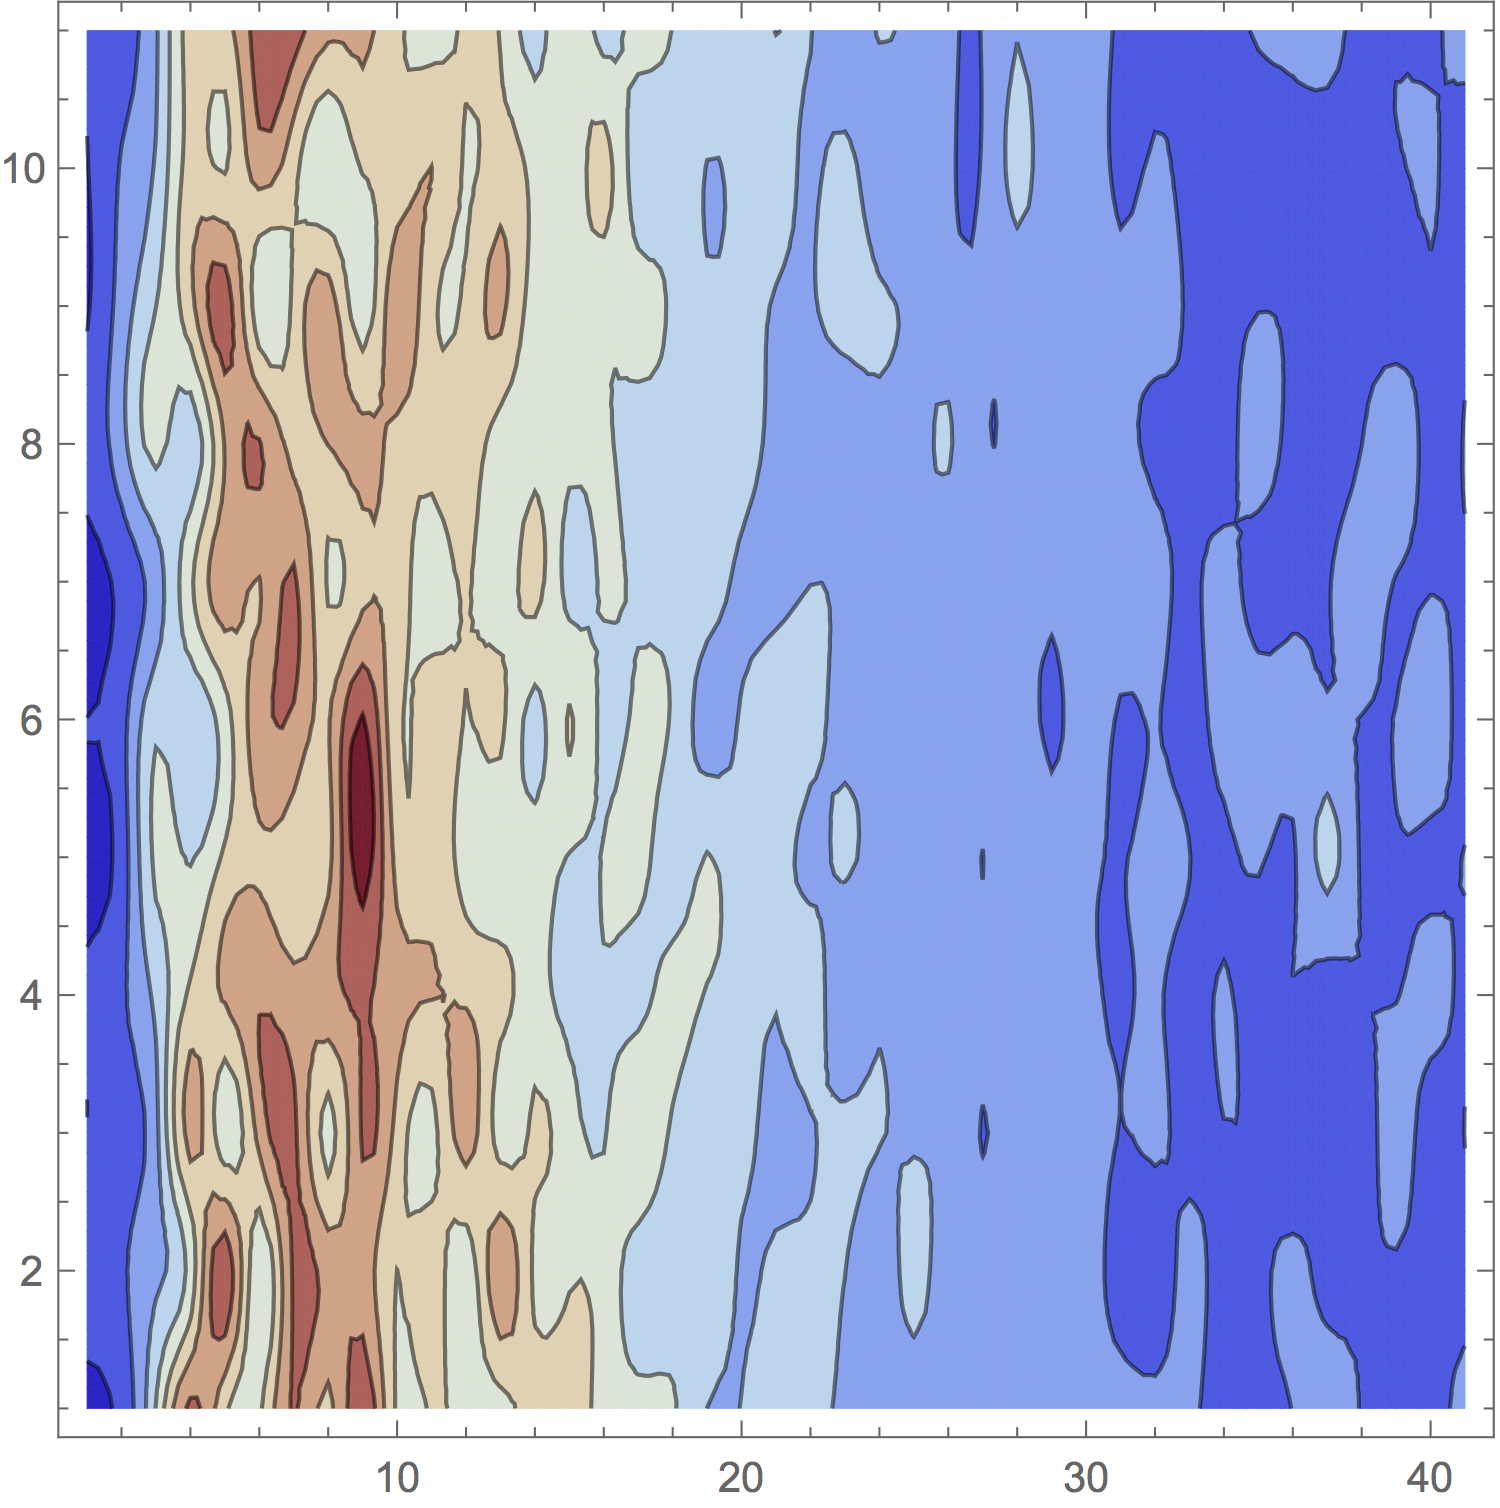
\includegraphics[scale=0.5]{efficiency_plot_col.png}
		\centering
		\caption{This plot shows the fidelity of the best organism in a ten-organism set after $100$ generations with respect to mutation chance and mutation magnitude. The vertical axis, when the value is multiplied by $0.1$, gives the chance in any generation for one of the angles defining an organism to be mutated. The horizontal axis, when multiplied by $0.025$, gives the mutation magnitude (this ranges between $0$ and $1$ radian(s)). The plot shows clear correlation between mutation magnitude and organism success.}
		\label{fig:effplot}
	\end{figure}

	Mutations are designated on the basis of chance and magnitude. We set a particular threshold value, which we are free to change. This threshold value ($\alpha$) determines whether or not a particular organism's parameters will be mutated. The parameters, as discussed above, are the $\beta '$ rotation coefficients which are specified in the exponential form of the local operations. The other changeable parameter, $\mu$, specifies the degree to which the angles will be mutated. These mutations encompass an envelope of random values between $-\mu$ and $\mu$  (a uniform distribution) which will be added to the current $\beta'$ values to update them.  Figure \ref{fig:effplot} depicts the efficacy of the simulation (particularly, the fidelity), for different values of $\alpha$ and $\mu$.  Lighter colors represent simulations resulting in higher fidelities. The values of $\alpha$ and $\mu$ do not change across the entire simulation; however, the efficiency of our program can be increased by modifying these values per each generation

	%%%%%%%%%%%%%%%%%%%%%%%%%%%%%%%%%%%%%%%%%%%%%%%%%%%%%%%

	\subsubsection{Classifying Fidelity and Breeding Operators} \label{breeding}

	We measure the fidelity of a matrix in a very conventional manner

	\begin{equation}
    \mathcal{F} = \frac{1}{|A - G|}
    \end{equation}

	where $A$ is a current matrix, and $G$ is a goal matrix that we hope to reach.  The magnitude of a matrix in this case is defined to be the square root of the sum of the squares of its elements.  The greater the fidelity, the closer the generated matrix is to the goal matrix.  

	When we breed two matrices together, we consider their individual fidelities $\mathcal{F}_1$ and $\mathcal{F}_2$.  We create the new parameters of a bred matrix based on the fidelities and angular parameters of the two parent matrices. Mathematically, this is given by a weighted average,

	\begin{equation}
    \beta_{breed}^{i} = \frac{\mathcal{F}_1\beta_{1}^{i} + \mathcal{F}_2\beta_{2}^{i}}{\mathcal{F}_1 + \mathcal{F}_2}
    \end{equation}
    
	where $i$ refers to all the relevant angular parameters. This will, given a sufficiently smooth space, allow the child organisms to retain properties of the parents, and fare better than if their mutations had been random, and each generation was composed of clones of the previous generation's most successful organisms. Note that in Figure \ref{fig:effplot}, the organisms were not subject to breeding. Despite this, we see remarkable success. 


	%%%%%%%%%%%%%%%%%%%%%%%%%%%%%%%%%%%%%%%%%%%%%%%%%%%%%%%

	\subsection{Convergence} \label{convergence}

	The search space is vast in this problem, increasing linearly in dimension with the increase of the number of generations, the number of organisms, and the number of genes in each organism. It is useful to determine which of these parameters is the most `volatile,' or increases the fidelity the largest amount with the smallest perturbation. 

	%%%%%%%%%%%%%%%%%%%%%%%%%%%%%%%%%%%%%%%%%%%%%%%%%%%%%%%

	\subsubsection{Variation in Population}

	A series of methods is used to determine fidelity in a populations of a set size, generation number, and gene length. We can then produce a series of partially-evaluated functions that can be mapped over a list of integers. When the results of this mapping are plotted, we gain knowledge of a slice of the search space. Knowledge of these slices, analogous to partial derivatives, can help determine which variables produce the best solutions with the smallest computational cost. 

	\begin{figure}[htpb]
		\centering
			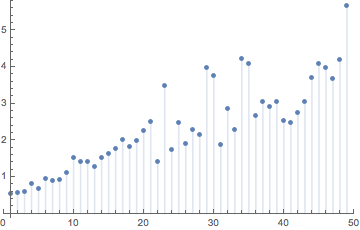
\includegraphics[scale=0.6]{20G_Plot_2.png}
		\centering
		\caption{A plot of the average of $20$ runs in which the population is along the horizontal axis, and fidelity ($\mathcal{F}$), is along the vertical axis. During these runs, the organism population was brought through $20$ generations, with each organism having two genes. The mutation chance ($\alpha$) and mutation magnitude ($\mu$) are drawn from the maximum of Figure \ref{fig:effplot} ($0.5$ and $0.225$ respectively).}
		\label{fig:pop_plot}
	\end{figure}

	Here we see a plot of constant generation number and gene length, where population size is being altered. Over a large average, the upward trend is clearly visible, as would make sense, and closely follows an exponential trend. We can conjecture that, given a saturation of the space with organism, we may eventually approach a point of diminishing returns, but that is not apparent in Figure \ref{fig:pop_plot}. These factors indicate a volatile variable, where we are sacrificing memory for some time and search space-covering. 

	%%%%%%%%%%%%%%%%%%%%%%%%%%%%%%%%%%%%%%%%%%%%%%%%%%%%%%%

	\subsubsection{Variation in Generation Number}

	The same process is used as described above, save now the slice through the search space is made in a way orthogonal to the original slice. On average, due to the structure of the space, the behavior along one slice is related to that at adjacent slices. We see a similar but not identical behavior. 

	\begin{figure}[htpb]
		\centering
			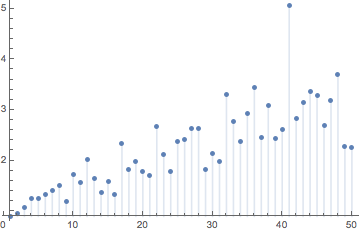
\includegraphics[scale=0.6]{20O_Plot_2.png}
		\centering
		\caption{A plot of the average of $20$ runs in which the generation number is along the horizontal axis, and fidelity is along the vertical. During this run, the number of generations is taken from $1$ to $50$, while the gene number remains at $2$, and the population is constant at $20$. ($\alpha$ and $\mu$ are preserved from Figure \ref{fig:pop_plot})}
		\label{fig:gen_plot}
	\end{figure}

	There is still a general upward trend when the data are aggregated. However, the growth with respect to generation number appears more logarithmic in character. This view is highlighted further in the paths along Figure \ref{fig:tot_plot}. These factors indicate that generation number is not as volatile a variable. 

	There are a number of explanations for this, but the most intuitive is that that size of the space is simply too large to be worked through by mutation alone. When there are few organisms, they stay within a close neighborhood of their original location (when breeding is not introduced, as it was not in these plots.) However, when the initial system is widely populated, each organism can work with the others to `patch' the space. 

	%%%%%%%%%%%%%%%%%%%%%%%%%%%%%%%%%%%%%%%%%%%%%%%%%%%%%%%

% 	\subsubsection{Variation in Gene Number}

% 	\begin{itemize}
% 	\item Absolute versus relative extrema
% 	\item Quality of metric
% 	\item Structure of the search space as a whole
% 	\item make tables with various independent variables
% 	\end{itemize}

	\subsubsection{The Space as a Whole}
    
    A key part to this algorithm's success is knowledge of the search space, and how mobility through it responds to variation in the parameters of its constituent functions. The first problem, explained and studied in \textbf{\ref{xx}.} is a helpful starting point for this analysis, as the solution is easily predicted. Figure \ref{fig:tot_plot} shows the fidelity, on average, of organisms in the $XX$ problem.

	\begin{figure}[htpb]
		\centering
			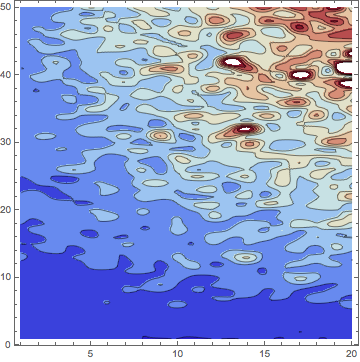
\includegraphics[scale=0.6]{genPlot_50O_20G.png}
		\centering
		\caption{This is a representation of the nature of the search space. Along the horizontal axis is generation number for the set of organisms, and along the vertical is the population of the set. The plot is taken as an average of 20 runs across the entire grid, with the contour plot interpolated between the data at each point; values shown are the fidelity of the best organism on average, and range from 0 to 6.}
		\label{fig:tot_plot}
	\end{figure}
    
    When adjusted for scale, two trends are evident in this plot. When population is held constant, representing a horizontal traversal of the plot, there is a relatively small variation in fidelity, while this gradient is increased greatly when traversal is made with generation number held constant. The contours in this plot are well defined, representing that the space is ordered and smooth, and a high-fidelity solution corresponds to nearby high-fidelity solutions.  

	%%%%%%%%%%%%%%%%%%%%%%%%%%%%%%%%%%%%%%%%%%%%%%%%%%%%%%%

	\subsection{Practicality and Caveats}

	In this scheme, there are a few pitfalls which may contribute to lack of success in finding a way to simulate the action of some Hamiltonian. The first is that this algorithm is non-deterministic, and with improper arguments, can have very little chance of producing a high-fidelity solution. Secondly, the algorithm is relatively greedy and naive, with solutions of higher fidelity always being chosen over those of lower, and against a metric that computes the direct norm between two operators' elements, rather than their actions. Finally, there are degeneracies in how the local operators are represented, as well as computational errors introduced by multiplication of high-precision numbers. 

	Each of the plots shown above is over an average of many runs. The nature of a random algorithm is to be random, and the inconsistencies in any one run can be accentuated if the population size or generation number is too small. In general, these numbers should be chosen to give consistently large fidelities (>$4$).

	The algorithm computes against a norm (described in \textbf{\ref{breeding}.}) that is a direct comparison, element by element, of two matrices. This is not directly akin to having two matrices act similarly, and serves as a poor heuristic when far from a solution. 

	Currently, the algorithm represents each unitary operator by a set of three angles (formalized in \textbf{\ref{arg}.}), with two ranging $[0, \pi)$ and the third from $[0, 2\pi)$. Given these restrictions, the angles experience a degeneracy, which may alter the overall phase of a solution's parts depending on when the angles are wrapped. 


%%%%%%%%%%%%%%%%%%%%___ RESULTS ___%%%%%%%%%%%%%%%%
%%%%%%%%%%%%%%%%%%%%%%%%%%%%%%%%%%%%%%%%%%%%%%%%%%%

			\section{Results and Data Analysis} \label{results}

	In the course of analysis of simulation schemes, there are certain cases of particular interest. The four we will study, which represent a good sample of the useful operations, are as follows: the $XX$ problem is an arbitrary but important (and easily verifiable) computation which maps from one operator to the same operator, the $XY$ problem, which attempts to go between simple expressions in the pauli basis, the $CNOT$ problem, which attempts to simulate a basic quantum gate, and the 0 problem, which attempts to simulate stasis, or the halting of evolution. 

	%%%%%%%%%%%%%%%%%%%%%%%%%%%%%%%%%%%%%%%%%%%%%%%%%%%%%%%

		\subsection{The $XX$ Problem} \label{xx}

	This problem represents a proof-of-concept. They purpose of this scheme is to generate complex unitary evolution operators, and not only is the problem

	\begin{empheq}[box=\fbox]{align}
		\mystrut{1em} exp\{\sigma_x \otimes \sigma_x\} \mapsto exp\{\sigma_x \otimes \sigma_x\}
	\end{empheq}

	attempting to represent a simple unitary evolution operator, it is attempting to represent the one we began with! Ideally, the results of a high-fidelity simulation in this case would yield identity matrices\footnote{Or $\sigma_x\otimes\sigma_x$, which produces the same result with two genes. Indeed, some of the solutions contained this alternate!}, and indeed, this would be the most efficient solution possible. To demonstrate trends in efficiency, we have produced a small table of fidelities, for example. 

	\begin{table}[htpb]
		\centering
			\begin{tabular}{||l | l l ||} 
			\hline
				Pop. & 20 Gen. & 50 Gen. \\ [0.5ex] 
			\hline
				10  & 0.63   & 0.95      \\ 
				25  & 0.86   & 1.71      \\
				50  & 1.17   & 2.17      \\
				100 & 4.79   & 2.31      \\
			\hline
			\end{tabular}
		\centering
		\caption{A chart of fidelities for the $XX$ problem. These values are not averaged, and give some feel as to the variations inherent to each trial.}
	\end{table}

	Apart from fidelity, the optimal organisms themselves may be analyzed. The algorithm, at the end of its search, provides the organism with the largest fidelity. This organism is represented by two lists, each containing the set of $A_i$ or $B_i$ as shown in (\ref{listEq}) in terms of three angles. These lists are then transformed back into traditional matrices, and combined to compare with the goal unitary operator. In a two-gene, 100 organism, 20 generation simulation, we can see that the generated matrix\footnote{The modulus of the entries has been taken for clarity, as the original matrix contained negligible imaginary parts. The values have also been truncated.} is very close to the predicted identity. 

	\begin{equation}
	A_1\otimes B_1 = 
	\begin{pmatrix}[1.3]
		{\color{crimson}\mathbf{0.99}}  &  0.08  &  0.01  &  0.00\\
		0.04  &  {\color{crimson}\mathbf{0.99}}  &  0.00  &  0.01\\
		0.01  &  0.00  &  {\color{crimson}\mathbf{0.99}}  &  0.08\\
		0.00  &  0.01  &  0.04  &  {\color{crimson}\mathbf{0.99}}
	\end{pmatrix}
	\end{equation}

	This simulation produced solid results because there exists a perfect solution that is easily predicted. There is no guarantee that, given a particular number of genes, a goal operator can be perfectly simulated \cite{victer}, only that more genes allows \emph{better} simulation. We expect to converge to more exotic goal operators slowly in comparison.

	%%%%%%%%%%%%%%%%%%%%%%%%%%%%%%%%%%%%%%%%%%%%%%%%%%%%%%%

	\subsection{The $XY$ Problem}

	In the interest of a less trivial problem, we attempt to move from a simple representation in one basis (represented by $X$, or the Hamiltonian $\sigma_x \otimes \sigma_x$), to another simple represented Hamiltonian ($\sigma_y \otimes \sigma_y$). We can represent this concisely by

	\begin{empheq}[box=\fbox]{align}
		\mystrut{1em} exp\{\sigma_x \otimes \sigma_x\} \mapsto exp\{\sigma_y \otimes \sigma_y\}
	\end{empheq}

	And can imagine how this can be extrapolated (through change of basis) to any tensor product of two local Hamiltonians. There are a few ways that this situation may be analyzed. The fidelities can be charted as done in the previous problem, or we may produce a larger chart of the space as in Figure \ref{fig:tot_plot}. 

	\begin{figure}[htpb]
		\centering
			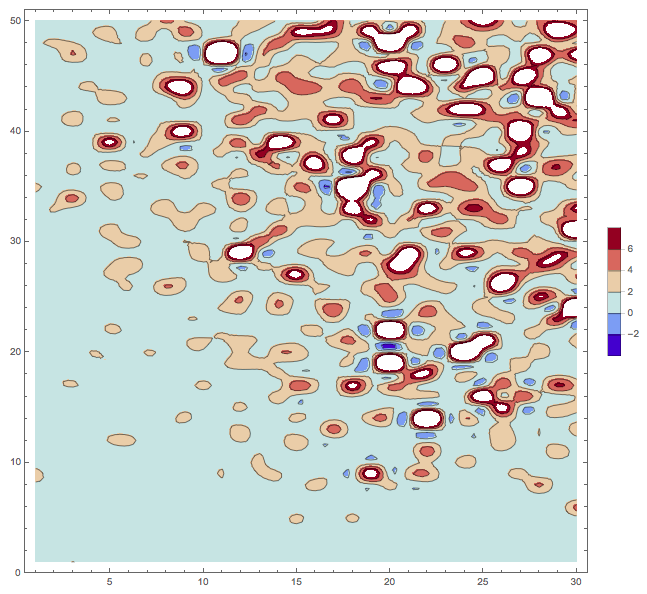
\includegraphics[scale=0.3]{xyPlot_50O_20G.png}
		\centering
		\caption{This shows the same plot as Figure \ref{fig:tot_plot}, but in the context of the $XY$ problem. A scale is included to show the fidelities. Note the absence of well defined contours.}
		\label{fig:xy_plot}
	\end{figure}

	In this chart, as opposed to the previous one, there are less well defined contours. This is due to the nature of the problem, in which the optimal solution is one that is more difficult to predict. The local operators here must not simply converge to identities, but coordinate their actions to bring a set rotation into another.
    
    As mentioned previously, we can also look at the operators generated from the best organism's set of angles (i.e. $A_1 \otimes B_1$ and $A_2 \otimes B_2$). Even general trends in these can be helpful in recognizing traits of solutions.

    \begin{figure}[htpb]
		\centering
			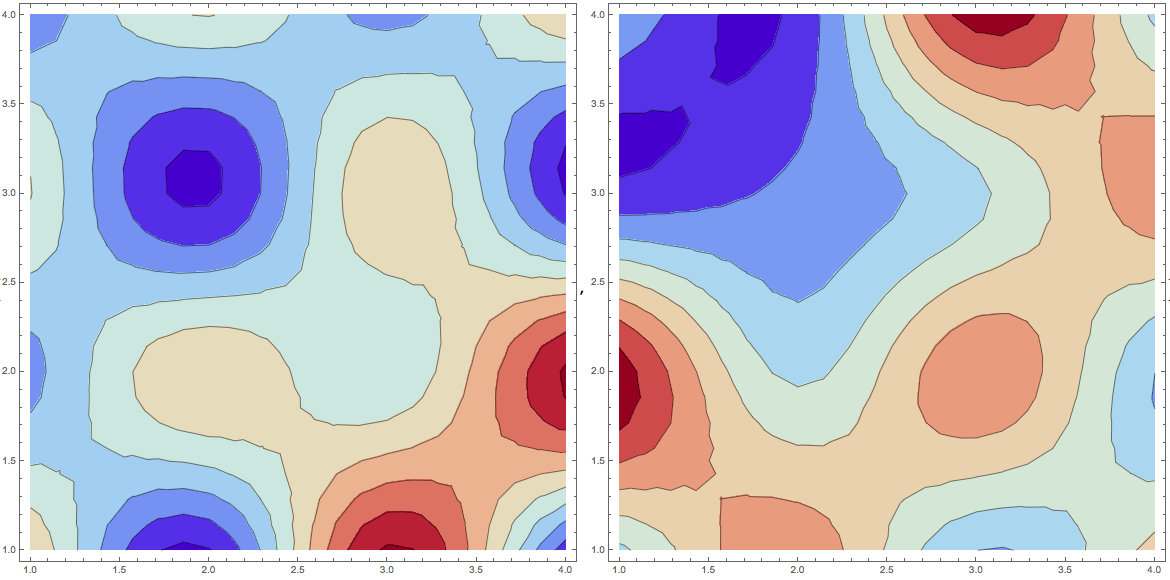
\includegraphics[scale=0.2]{xy_test_matrices.png}
		\centering
		\caption{A contour plot of the local operations ($A_i \otimes B_i$) performed by an organism in the $XY$ problem. Note that this is an interpolation of a matrix's elements (a four by four grid) and is therefore a useful heuristic, rather than a concrete tool for analysis. The modulus value of the entries were taken, and thus phase factors are lost.}
		\label{fig:xy_matrix}
	\end{figure}

	For example, in Figure \ref{fig:xy_matrix}, we see that the concentration of value in the local operators is not along the diagonal, as was the case in the $XX$ problem, but instead concentrated in the lower or upper off-diagonals. Patterns such as these, and alternative ones developed in the same problem\footnote{See appendix for alternative pattern.}, can give useful hints. 

	In these types of problems, high fidelities can be reached, but the algorithm is less stable, and generally requires a larger population to produce similar quality. 
	

	%%%%%%%%%%%%%%%%%%%%%%%%%%%%%%%%%%%%%%%%%%%%%%%%%%%%%%%

	\subsection{The $CNOT$ Problem}

	\begin{empheq}[box=\fbox]{align}
		\mystrut{1em} exp\{\sigma_x \otimes \sigma_x\} \mapsto CNOT
	\end{empheq}

	The purpose of this simulation scheme is to generate methods to create useful quantum operators. These manifest in the canonical quantum gates. Among the most notorious of these (and from which all others can be constructed \cite{oliviera}) is the $CNOT$ gate, represented in matrix form as such

	\begin{equation}
	CNOT = 
	\begin{pmatrix}[1.1]
		1  &  0  &  0  &  0  \\
		0  &  1  &  0  &  0  \\
		0  &  0  &  0  &  1  \\
		0  &  0  &  1  &  0 
	\end{pmatrix}
	\end{equation}

	This operator allows one qubit's state to affect the operation applied to another. This is incredibly pertinent in control theory. By the nature of the correlation it implies between particles, this operator is not the tensor product of two local operators. Due to this, the non-local piece of the initial Hamiltonian must take the brunt of the work in producing $CNOT$. 

	Initial runs yield exotic matrix plots 
	
	\begin{figure}[htpb]
		\centering
			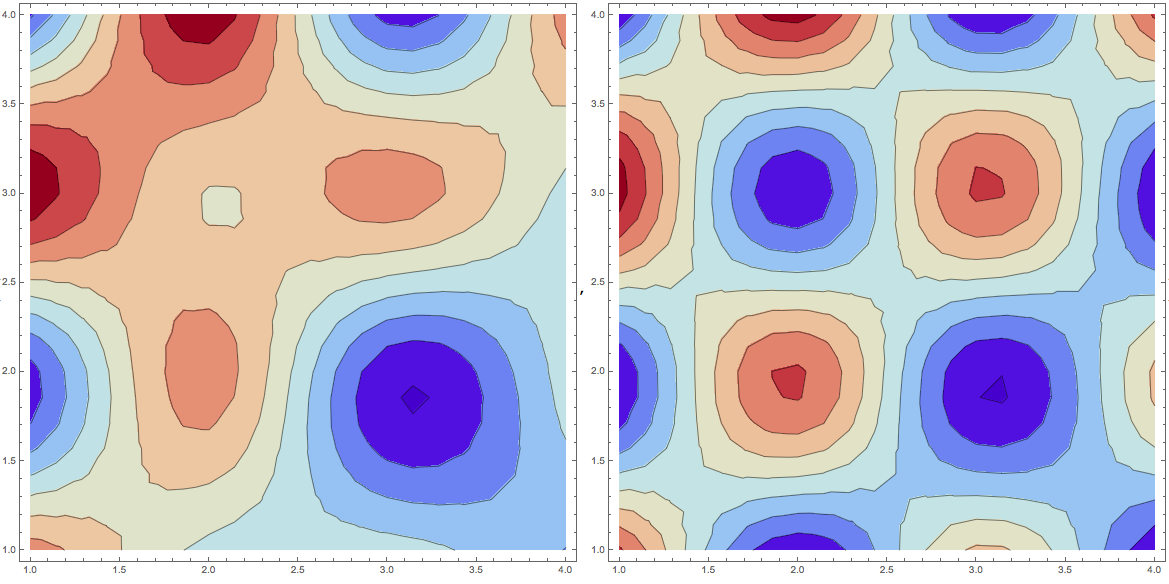
\includegraphics[scale=0.2]{cnot_matrices.png}
		\centering
		\caption{Plots of the LO for the $CNOT$ problem. Note that the operators are markedly different, but maintain a concentration of value in the upper off-diagonals.}
		\label{fig:cnot_matrix}
	\end{figure}

	However, the difficulty of simulating this operator manifests itself in relatively low fidelities given the same generation and population numbers used in the previous problems. There are a few possible ways to increase fidelity (or rather, the potential fidelity) of $CNOT$ simulations.

	The discrete times during which the initial Hamiltonian is applied between LO can be varied so as to increase the mobility of the non-local evolution. Alternatively, more genes could be introduced into the test organisms, allowing more local operations across the total evolution. Unfortunately, both of these options increase runtime dramatically if the algorithm is not run in parallel. The fidelity we are able to achieve readily with the base algorithm ($\approx3$) is sufficient for our purposes. 

	%%%%%%%%%%%%%%%%%%%%%%%%%%%%%%%%%%%%%%%%%%%%%%%%%%%%%%%

	\subsection{The 0 Problem}

	Although there are many simulations possible that are useful to control theory, the final example will be in the simulation of the zero-Hamiltonian, or the stasis of a system. Engineering dynamic Hamiltonians has distinct uses, but preserving the state of the system is unique in two respects: it represents the negation of the original Hamiltonian, and it allows the state of a system to be preserved indefinitely. The problem is represented as such (the zero-Hamiltonian produces the identity as its unitary evolution operator). 

	\begin{empheq}[box=\fbox]{align} \label{identity}
		\mystrut{1em} exp\{\sigma_x \otimes \sigma_x\} \mapsto \mathds{1}
	\end{empheq}

	To give a feel for the fidelity, below is a sampled unitary evolution operator approximation from an average run at 100 organisms and 20 generations. 

	\begin{equation}
	\tilde{U} = 
	\begin{pmatrix}[1.1]
		{\color{crimson}\mathbf{0.86}}   &  0.07  &  0.07  &  0.10  \\
		0.07  &  {\color{crimson}\mathbf{0.86}}   &  0.09  &  0.07  \\
		0.17  &  0.10  &  {\color{crimson}\mathbf{1.08}}   &  0.15  \\
		0.10  &  0.17  &  0.14  &  {\color{crimson}\mathbf{1.08}}  
	\end{pmatrix}
	\end{equation}

	Note that this does not enjoy the luxuries\footnote{Equation \ref{identity} is not the unitary evolution operator, but rather a single LO.} of (\ref{identity}), but is still recognizable with its concentration on the diagonal. Over the course of runs in the 0 problem, it was found that consistent convergences were difficult to manage, and often required much larger populations to compensate. This is to be expected, given that the goal is to reverse an arbitrary non-local Hamiltonian's actions. As a side note, the solutions of high fidelity were found to have drastically different structure, implying once more that there are various `families' of solutions that, if they are not equally efficient, serve as local extrema in the search space. 

	%%%%%%%%%%%%%%%%%%%%%%%%%%%%%%%%%%%%%%%%%%%%%%%%%%%%%%%

	\subsection{The Effectiveness of Breeding}
	
	In all of the above problem, there comes the question of how to best move organisms through the search space. The primary methods by which this is altered are (1) how the organisms mutate, and (2) how the organisms (if it is enabled) breed with one another. Both have shown to be important in the simulations, and less intuitive than originally considered. 

	Mutations in the organisms are controlled by two factors, $\alpha$ and $\mu$, or the probability of mutation, and the magnitude bounds if it does occur. In essence, these help to define the `radius' that a lone organism may traverse over its lifetime. The organism must not be stagnant, lest it explore none of the space around it, and must also not mutate wildly, lest it jump randomly around the space with no sense of increasing fidelity in any one direction. The nature of our tests show that focus on continuity is more important than exploring the entire space, and so smaller mutations allow for better overall solutions with regards to one organism. 

	However, when one cannot explore the entire space, the extrema to be found are limited by generation number and luck. More organisms to `patch' the space are the most efficient way to tackle this, but handling this increase in population is computationally expensive. 

	The ostensible solution to this problem is to breed the organisms, and this is described in \textbf{\ref{breeding}.} When this process was implemented, however, there was not an amazing increase in fidelity. The reason conjectured for this is relatively simple. In breeding, the organisms `pull' towards one another to produce offspring, with the child organism closer to the better parent. The weight is based on the relative magnitudes of the fidelities, and thus even rather poorly performing parents can draw all future organisms near them in a couple generations. This induces the problem mentioned previously. Ideally, the breeding would be rewritten to correct this premature convergence. 
	

%%%%%%%%%%%%%%%%%%%%___ CONCL _____%%%%%%%%%%%%%%%%
%%%%%%%%%%%%%%%%%%%%%%%%%%%%%%%%%%%%%%%%%%%%%%%%%%%

	\section{Conclusion}

We have identified various aspects of using adaptive algorithms that are beneficial and detrimental in determining local operation sets to simulate an arbitrary gate. Although Our results have consistently agreed mathematically, with fairly large fidelity, the run-time grows exponentially with the number of organisms, generations, and gene number. This can only be countered well by running this program with multiple processors (i.e. in parallel, which this algorithm is well-suited for) \cite{umbarkar}. Moreover, a lot of lag in the code is derived from matrix multiplication, which is a daunting task to optimize. Perhaps, using a more effective algorithm will improve the run-time efficiency of the code as well. We can however partially ease matrix multiplication by taking advantage of particular expansions of matrix exponentials, which can be truncated depending upon our desired accuracy. Using commutation relations and Lie algebras may immensely help with the reduction of run-time as well (this involves both engineering the heuristic and the initial populations). The methods forming the basis of this scheme are naive, and base little of their workings off of the defining tricks of linear algebra and group theory. There are properties to be exploited, but we chose to produce a functional process before an optimal one. We also wish to represent better ways of representing the resulting operators, to give more intuition about their structure.

Although we compromise time for efficiency, our efforts in implementing adaptive algorithms to solve this quantum computation problem has yielded high success in producing a viable solution sets. With complex systems, as are necessary to produce non-trivial quantum computations, analytical methods for generating the correct unitary evolution operator are simply not feasible. With the proper improvements, non-deterministic methods such as the one here are vital to the success of quantum computation. 

%%%%%%%%%%%%%%%%%%%%___ APPEND _____%%%%%%%%%%%%%%%
%%%%%%%%%%%%%%%%%%%%%%%%%%%%%%%%%%%%%%%%%%%%%%%%%%%

	\section{Appendix} \label{appendix}

	%%%%%%%%%%%%%%%%%%%%%%%%%%%%%%%%%%%%%%%%%%%%%%%%%%%%%%%

	\subsection{Condensed Operator Syntax}

	As shown in \textbf{\ref{arg}.} we define a notation for a linear combination of the pauli- and identity-matrices through a quasi-dot-product, where $\beta$ is defined as some vector in $\mathbb{C}^4$, and its product with the extended sigma vector is defined as

	\begin{align*}
		\beta \cdot \sigma &= \beta_0\, \mathds{1} + \beta_1\, \sigma_1 + \beta_2\, \sigma_2 + \beta_3\, \sigma_3\\[3mm]
		\sigma_1 &= 
		\begin{pmatrix}
			0 & \;\;1\\[1mm]
			1 & \;\;0
		\end{pmatrix}
		\;
		\sigma_2 = 
		\begin{pmatrix}
			0 & -i\\[1mm]
			i & 0
		\end{pmatrix}
		\\[3mm]
		\sigma_3 &= 
		\begin{pmatrix}
			1 & 0\\[1mm]
			0 & -1
		\end{pmatrix}
	\end{align*}

	In the second case, where $\beta'$ is used for the quasi-dot-product, we can consider $\beta'$ as a vector in a subspace of $\mathbb{C}^4$ with the first element $0$, or as a vector in $\mathbb{C}^3$, with $\sigma$ modified to accommodate the product. Regardless, we have that

	\begin{equation*}
	\beta' \cdot \sigma = \beta_1'\, \sigma_1 + \beta_2'\, \sigma_2 + \beta_3'\, \sigma_3
	\end{equation*}

	With the same definitions for the pauli-matrices as shown above.
    
    \subsection{Alternative $XY$ Problem Solution}

	\begin{figure}[htpb]
		\centering
			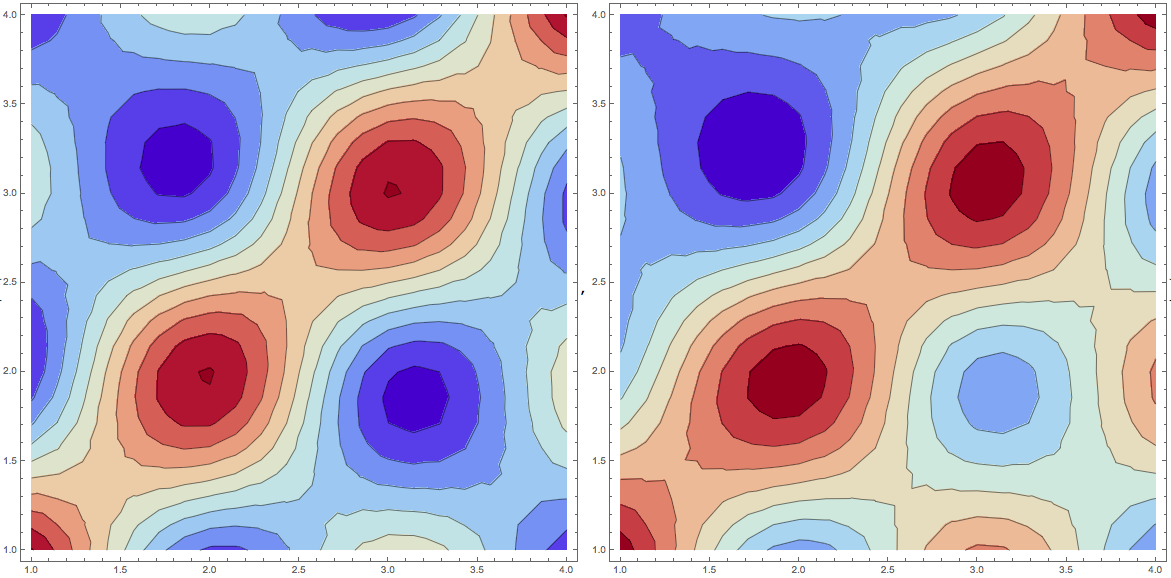
\includegraphics[scale=0.2]{xy_alt_matrices.png}
		\centering
		\caption{A contour plot of the local operations performed by an organism in the $XY$ problem. Note that now the large-modulus terms are along the opposite diagonal to those emphasized in the $XX$ problem.}
		\label{fig:xy_alt}
	\end{figure}



%%%%%%%%%%%%%%%%%%%%___ BIBLIO _____%%%%%%%%%%%%%%%
%%%%%%%%%%%%%%%%%%%%%%%%%%%%%%%%%%%%%%%%%%%%%%%%%%%
				\bibliographystyle{plain}
				\bibliography{ref}
               



\end{document}